

\title{ PyDash Requirements Document  \\ 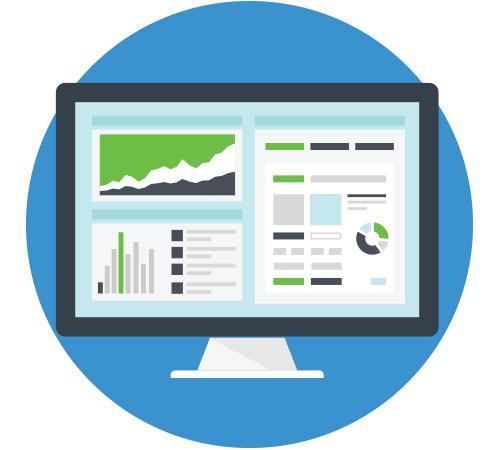
\includegraphics[width=2.50746in,height=2.26563in]{media/image2.jpg}}

\begin{longtable}[]{@{}ll@{}}
\toprule
\endhead
\begin{minipage}[t]{0.47\columnwidth}\raggedright
\textbf{PyDash 2018}

J. G. S. Overschie

T. W. E. Apol

A. Encinas-Rey Requena

K. Bolhuis

W. M. Wijnja

L. J. Doorenbos

J. Langhorst

A. Tilstra\strut
\end{minipage} & \begin{minipage}[t]{0.47\columnwidth}\raggedright
\textbf{Customers}

Patrick Vogel

Mircea Lungu

\textbf{TA}

Patrick Vogel\strut
\end{minipage}\tabularnewline
\bottomrule
\end{longtable}

\today

\pagebreak

\tableofcontents


\hypertarget{introduction}{%
\section{Introduction}\label{introduction}}

For implementing web services using Python, one of the most used
solutions is called Flask. This however does not include a way to
monitor which parts of the web service are used at what rate. A
dashboard able to collect this data was developed by a group of
computing science students of the University of Groningen. There are
still a few shortcomings in this dashboard, most notably in the case of
monitoring a large number of Flask apps.

To solve this, PyDash.io can be used. PyDash.io is a dashboard
containing the information of multiple deployed Flask monitoring
dashboards. The user (with the right credentials) now has a better
overview of his deployed dashboards, and does not have to maintain
multiple credentials for each one.

\hypertarget{target-users}{%
\section{Target Users}\label{target-users}}

Administrators of web services/API's. This users are a potential target
as it will be very interested to make possible that other companies,
apart from RUG, make use of the system. It would be useful for them to
be able to measure with the analytic system the number of hits in their
website. The system can be used as a global measurement or more
specific. This will also benefit companies as they will be able to
measure a certain part of the website and view what customers are
interested when entering in their pages. So, this will mean that they
will be able to correct errors of their websites or even improve and
make emphasis on what their customers like.

Developers. As well as for the Administrators of web services/API's, the
Developers will be able to take advantages of the system to develop a
dashboard. The dashboard will offer the developers to measure the
effectiveness of their websites. Developers will be able to create a
tool that will help them to improve their websites. So, as well as for
Administrators, the system will help Developers to correct errors but
also, to develop a effective system for their dashboards.

\hypertarget{section-2}{%
\section{\texorpdfstring{\\
}{ }}\label{section-2}}

\hypertarget{requirements}{%
\section{Requirements}\label{requirements}}

\hypertarget{high-priority}{%
\subsection{High Priority}\label{high-priority}}

\begin{itemize}
\item
  \begin{quote}
  Users need to be able to create an account.
  \end{quote}
\item
  \begin{quote}
  Users need to be able to log in to their account.
  \end{quote}
\item
  \begin{quote}
  Users need to be able to register flask-monitoring-dashboards.
  \end{quote}
\item
  \begin{quote}
  Users need to be able to see an overview of all their registered
  dashboards.
  \end{quote}
\item
  \begin{quote}
  The PyDash service needs to receive data from each registered
  dashboard in regular intervals, for example, on an hourly basis.
  \end{quote}
\item
  \begin{quote}
  For each registered dashboard: Functionality for users to change which
  endpoints are being monitored.
  \end{quote}
\item
  \begin{quote}
  For each registered dashboard: visualising (the performance of) said
  dashboard\\
  (similar to how a dashboard is currently visualised):
  \end{quote}

  \begin{itemize}
  \item
    \begin{quote}
    Overview of dashboard (all included endpoints):
    \end{quote}

    \begin{itemize}
    \item
      \begin{quote}
      Graph of summed endpoint executions (per hour)
      \end{quote}
    \item
      \begin{quote}
      A set of horizontal bar-plots of how many times Endpoints are
      executed per day
      \end{quote}
    \item
      \begin{quote}
      Execution time - all endpoints and versions:
      \end{quote}

      \begin{itemize}
      \item
        \begin{quote}
        Per version:\\
        Show a horizontal box-plot of the execution times (over all
        Endpoints) per version
        \end{quote}
      \item
        \begin{quote}
        Per endpoint:\\
        Show a horizontal box-plot of the execution times per Endpoint
        (over all versions)
        \end{quote}
      \end{itemize}
    \end{itemize}
  \end{itemize}
\item
  \begin{quote}
  There should also be endpoint specific pages that show more detailed
  information:
  \end{quote}

  \begin{itemize}
  \item
    \begin{quote}
    Endpoint summary/overview:
    \end{quote}

    \begin{itemize}
    \item
      \begin{quote}
      Endpoint name
      \end{quote}
    \item
      \begin{quote}
      Added since app version (version nr.)
      \end{quote}
    \item
      \begin{quote}
      Date added to app (date \& time)
      \end{quote}
    \item
      \begin{quote}
      Link to endpoint
      \end{quote}
    \item
      \begin{quote}
      Last accessed (date \& time)
      \end{quote}
    \end{itemize}
  \item
    \begin{quote}
    Execution time:
    \end{quote}

    \begin{itemize}
    \item
      \begin{quote}
      Per day:
      \end{quote}

      \begin{itemize}
      \item
        \begin{quote}
        Show a stacked-vertical-bar-plot with the average execution time
        per day.
        \end{quote}
      \end{itemize}
    \item
      \begin{quote}
      Per user, per version:\\
      Show a dot-plot for the average execution time per user per
      version.
      \end{quote}
    \item
      \begin{quote}
      Per IP-address, per version:\\
      Show a dot-plot for the average execution time per IP-address per
      version.
      \end{quote}
    \item
      \begin{quote}
      Per version:\\
      Show a box-plot for the execution time per version.
      \end{quote}
    \item
      \begin{quote}
      Per user:
      \end{quote}

      \begin{itemize}
      \item
        \begin{quote}
        Show a box-plot for the execution time per user.
        \end{quote}
      \end{itemize}
    \end{itemize}
  \item
    \begin{quote}
    Hits per day:
    \end{quote}

    \begin{itemize}
    \item
      \begin{quote}
      Vertical-bar-plot:\\
      Show a vertical-bar-plot with the number of hits per day.
      \end{quote}
    \item
      \begin{quote}
      Heatmap:\\
      Show a heatmap (per hour) when the specific Endpoint was executed.
      \end{quote}
    \end{itemize}
  \end{itemize}
\end{itemize}

\hypertarget{low-priority}{%
\subsection{Low Priority}\label{low-priority}}

\begin{itemize}
\item
  \begin{quote}
  For each registered dashboard visualising (the performance of) said
  dashboard:
  \end{quote}

  \begin{itemize}
  \item
    \begin{quote}
    Endpoint specific:
    \end{quote}

    \begin{itemize}
    \item
      \begin{quote}
      Debug info about potential outliers:
      \end{quote}

      \begin{itemize}
      \item
        \begin{quote}
        Date (date \& time)
        \end{quote}
      \item
        \begin{quote}
        Execution time (in ms)
        \end{quote}
      \item
        \begin{quote}
        Request values
        \end{quote}
      \item
        \begin{quote}
        Request headers
        \end{quote}
      \item
        \begin{quote}
        Request environment
        \end{quote}
      \item
        \begin{quote}
        Request url
        \end{quote}
      \item
        \begin{quote}
        Cpu percent
        \end{quote}
      \item
        \begin{quote}
        Memory
        \end{quote}
      \item
        \begin{quote}
        Stacktrace
        \end{quote}
      \end{itemize}
    \end{itemize}
  \end{itemize}
\item
  \begin{quote}
  A number of static tutorial pages, detailing how to use the
  flask-monitoring-dashboard.
  \end{quote}
\item
  \begin{quote}
  An administrator overview for PyDash.io, where an administrator can
  see visualizations on the usage of PyDash.io itself.
  \end{quote}

  \begin{itemize}
  \item
    \begin{quote}
    In order to do this, we deploy a flask-monitoring-dashboard on
    PyDash.io itself.
    \end{quote}
  \end{itemize}
\item
  \begin{quote}
  Allow users to change scope of monitored endpoints in case there are
  many. e.g. hiding or showing endpoints or groups of endpoints.
  \end{quote}
\end{itemize}

\hypertarget{nice-to-have}{%
\subsection{Nice to have}\label{nice-to-have}}

\begin{itemize}
\item
  \begin{quote}
  In the future, we might want to support other types of dashboards,
  such as, for example, a django-monitoring-dashboard.
  \end{quote}
\item
  \begin{quote}
  Allow users to enable/disable the actual monitoring of specific
  endpoints. \emph{\textbf{Since the flask-monitoring-dashboard API does
  not yet provide any way to achieve this, we will not yet be able to
  implement this feature.}}
  \end{quote}
\end{itemize}

\hypertarget{not-going-to-build}{%
\subsection{Not going to build}\label{not-going-to-build}}

\begin{itemize}
\item
  \begin{quote}
  Add more visualizations.
  \end{quote}

  \begin{itemize}
  \item
    \begin{quote}
    We will most likely not add more visualizations than
    \emph{flask-monitoring-dashboard} currently includes.
    \end{quote}
  \end{itemize}
\end{itemize}

\hypertarget{non-functional-requirements}{%
\section{Non-functional
requirements}\label{non-functional-requirements}}

\hypertarget{high-priority-1}{%
\subsection{High priority}\label{high-priority-1}}

\begin{itemize}
\item
  \begin{quote}
  Security + Privacy
  \end{quote}

  \begin{itemize}
  \item
    \begin{quote}
    We want to use an Secure Socket Layer connection, both to connect
    the users to the application, as well as to connect to the different
    instances of the \emph{flask-monitoring-dashboard}. The reasoning
    behind this, is that when we do not do this, sensitive information
    might be shared or stolen with third parties.
    \end{quote}
  \item
    \begin{quote}
    We want to hash the user-account passwords in the application, to
    ensure that in the unfortunate event that PyDash.IO's information
    might be compromised, that the user accounts are relatively safe.
    \end{quote}
  \item
    \begin{quote}
    We want to prevent the resources used in the application to be
    susceptible to an \emph{enumeration} attack: That is, authorization
    to access a certain resource will be checked before returning it,
    and inside URLs, identifiers that are non-incrementing integers will
    be used. This will stop people from both getting insight into the
    data we have stored by looking at the identifiers (for example how
    many dashboards we have) and using the URL syntax to access new
    endpoints they would otherwise not know about.
    \end{quote}
  \end{itemize}
\item
  \begin{quote}
  Tooling
  \end{quote}

  \begin{itemize}
  \item
    \begin{quote}
    Usage of the programming language Python and the micro web framework
    Flask is required to build the PyDash.IO application. The reason
    behind this is to be able to use the
    \emph{flask-monitoring-dashboard} to monitor the PyDash.IO web
    application itself at some point.
    \end{quote}
  \end{itemize}
\end{itemize}

\hypertarget{low-priority-1}{%
\subsection{Low priority}\label{low-priority-1}}

\begin{itemize}
\item
  \begin{quote}
  Responsive Design: We want the application to function properly (do
  not have lacking functionality) and not contain obvious graphical bugs
  or oversights. We are going to test this by accessing our web tool on
  different systems. We want our tool to work on at least the following
  display sizes:
  \end{quote}

  \begin{itemize}
  \item
    \begin{quote}
    A Full-HD screen (1920 x 1080)px
    \end{quote}
  \item
    \begin{quote}
    A medium-sized computer or tablet screen (1280 x 768)px
    \end{quote}
  \item
    \begin{quote}
    A small portrait-mode smartphone screen (320 x 550)px
    \end{quote}
  \end{itemize}
\item
  \begin{quote}
  Scalability
  \end{quote}

  \begin{itemize}
  \item
    \begin{quote}
    In the hopes that PyDash.IO will be used by a reasonable group of
    users at some point, we want to ensure that the application can
    handle at least fifty \emph{flask-monitoring-dashboard} instances
    side-by-side without the application being hampered in its primary
    purpose, which is to have users browse the distilled information
    already extracted from those \emph{flask-monitoring-dashboards.} An
    endpoint response is too slow for a user if it takes longer than 0.5
    seconds to respond, measured in server execution time.
    \end{quote}
  \end{itemize}
\item
  \begin{quote}
  Etiquette of performing external API calls
  \end{quote}

  \begin{itemize}
  \item
    \begin{quote}
    When calling into an external \emph{flask-monitoring-dashboard}, it
    is mandatory to not stress (overload) that application too much.
    This means that we need to rate-limit the calls made to these
    external applications (Do not perform a request to the same
    application more often than once every three minutes), as well as
    ensure that we do not request too much data at one time from them.
    \end{quote}
  \end{itemize}
\end{itemize}


\hypertarget{finished-backlog-tasks}{%
\section{Finished backlog tasks}\label{finished-backlog-tasks}}

\hypertarget{sprint-4}{%
\subsection{Sprint 4}\label{sprint-4}}

\emph{Backend}

\begin{itemize}
\item
  \begin{quote}
  Fetching fixed
  \end{quote}

  \begin{itemize}
  \item
    \begin{quote}
    Due to concurrency issues and Wiebe-Marten not being available to
    help out, we did not manage to get periodic background fetching to
    work. For this reason, currently dashboard data is fetched everytime
    the dashboard page is loaded.
    \end{quote}
  \item
    \begin{quote}
    By Sprint \#4, periodic fetching needs to be working.
    \end{quote}
  \end{itemize}
\item
  \begin{quote}
  Better error handling when fetching
  \end{quote}

  \begin{itemize}
  \item
    \begin{quote}
    While fetching works at the moment, error handling needs to be
    improved since there are some edge cases where an error is raised
    and the application crashes.
    \end{quote}
  \end{itemize}
\item
  \begin{quote}
  Account creation
  \end{quote}

  \begin{itemize}
  \item
    \begin{quote}
    An API route needs to be added to support account creation; this
    will put the new user in a "waiting for confirmation" state and
    generate a verification code.
    \end{quote}
  \item
    \begin{quote}
    An API route needs to be added for email verification based on a
    given code.
    \end{quote}
  \item
    \begin{quote}
    Sending emails, and the frontend UI, will be done in Sprint \#5.
    \end{quote}
  \end{itemize}
\item
  \begin{quote}
  Continuous Integration (CI) and deployment
  \end{quote}

  \begin{itemize}
  \item
    \begin{quote}
    Set up testing and continuous integration of the backend
    application.
    \end{quote}
  \item
    \begin{quote}
    Deploy the entire application to the server.
    \end{quote}
  \item
    \begin{quote}
    Arrange TLS/SSL.
    \end{quote}
  \end{itemize}
\end{itemize}

\emph{Frontend}

\begin{itemize}
\item
  \begin{quote}
  Account creation
  \end{quote}

  \begin{itemize}
  \item
    \begin{quote}
    A register account button has to be added to the current login page
    which directs the user to the register account page.
    \end{quote}
  \item
    \begin{quote}
    The register account page has to be made, containing fields for
    name, e-mail, password and verify password which when all properly
    filled in will create the new account.
    \end{quote}
  \end{itemize}
\item
  \begin{quote}
  Add more graphs
  \end{quote}

  \begin{itemize}
  \item
    \begin{quote}
    Visualizations have to be added to the individual dashboard pages
    and the individual endpoint pages, containing information about
    among others number of endpoint visits and last access time. In this
    sprint we will aim for at least three different graphs per dashboard
    page, namely a graph for visits per day, unique visitors per day,
    and endpoint popularity.
    \end{quote}
  \end{itemize}
\item
  \begin{quote}
  Revise the overview page
  \end{quote}

  \begin{itemize}
  \item
    \begin{quote}
    The overview currently contains a graph and a name per dashboard,
    this has to be changed to containing just the name and a simple
    statistic such as total number of visits in the last week. Each tile
    is then a link to the individual page of said dashboard.
    \end{quote}
  \end{itemize}
\item
  \begin{quote}
  Implement basis for adding and removing dashboards from the overview
  page
  \end{quote}

  \begin{itemize}
  \item
    \begin{quote}
    As this is a lot of work for just sprint 5, the basis can be built
    here. Think of adding the necessary buttons or designing the
    verification of the url and secret token.
    \end{quote}
  \end{itemize}
\item
  \begin{quote}
  Implement endpoint specific page
  \end{quote}

  \begin{itemize}
  \item
    \begin{quote}
    Not only is it possible to view the data of a dashboard, there is
    also a page with statistics for every endpoint of that dashboard,
    accessed through the dashboard overview page. This endpoint page has
    to be created and the proper links have to be added to the dashboard
    pages. The design for the endpoint page can be found in the design
    folder of the google drive.
    \end{quote}
  \item
    \begin{quote}
    On this page multiple cards must be displayed. The top one when
    opened shows general data about the endpoint, and the other cards
    all consist of graphs.
    \end{quote}
  \end{itemize}
\end{itemize}

\hypertarget{sprint-5}{%
\subsection{Sprint 5}\label{sprint-5}}

\emph{Backend}

\begin{itemize}
\item
  \begin{quote}
  Make error messages more user friendly
  \end{quote}

  \begin{itemize}
  \item
    \begin{quote}
    Right now, the error messages are simply Python exceptions: we need
    to make this more user friendly.
    \end{quote}
  \end{itemize}
\end{itemize}

\begin{itemize}
\item
  \begin{quote}
  Implement email verification
  \end{quote}

  \begin{itemize}
  \item
    \begin{quote}
    The meat of the functionality is already in place (generating a code
    and the API route to verify it). We still need to send actual
    emails.
    \end{quote}
  \end{itemize}
\item
  \begin{quote}
  Implement adding and removing dashboards
  \end{quote}

  \begin{itemize}
  \item
    \begin{quote}
    For example, add new routes to add and remove a dashboard.
    \end{quote}
  \item
    \begin{quote}
    Alternatively, use the PUT and DELETE HTTP methods to indicate
    intention.
    \end{quote}
  \end{itemize}
\item
  \begin{quote}
  Implement user settings
  \end{quote}

  \begin{itemize}
  \item
    \begin{quote}
    Define user settings
    \end{quote}
  \item
    \begin{quote}
    Routes to retrieve, update and delete user settings need to be
    added.
    \end{quote}
  \item
    \begin{quote}
    Alternatively, this could be done using HTTP verbs on existing
    routes.
    \end{quote}
  \end{itemize}
\item
  \begin{quote}
  Revise aggregator issue \#105.3
  \end{quote}
\end{itemize}

\emph{Frontend}

\begin{itemize}
\item
  \begin{quote}
  Implement adding and removing dashboards from the overview page.
  \end{quote}

  \begin{itemize}
  \item
    \begin{quote}
    Addition will be done by clicking on a plus in the top right corner
    of the overview page. When clicked the user will be able to fill in
    the dashboard url, its name and the secret token associated with
    that dashboard. If correctly filled in, the dashboard will be added
    as a tile to the users overview page.
    \end{quote}
  \item
    \begin{quote}
    Removing is done by clicking on a three dot sign present in the
    bottom left corner of every dashboard page. When clicked, the user
    will be asked to confirm his action after which the dashboard is
    permanently removed from the overview page.
    \end{quote}
  \end{itemize}
\item
  \begin{quote}
  Implement user settings
  \end{quote}

  \begin{itemize}
  \item
    \begin{quote}
    When clicking on the tab Settings, currently already present in the
    menu, the user will be redirected to the Settings page
    \end{quote}
  \item
    \begin{quote}
    The settings page has to be made, containing settings such as
    changing your password, the email account associated with the user,
    or account deletion.
    \end{quote}
  \end{itemize}
\item
  \begin{quote}
  Add more graphs
  \end{quote}

  \begin{itemize}
  \item
    \begin{quote}
    As we will probably not be able to implement all the different
    visualisations we want during sprint 4, the rest or another part of
    them will be added during sprint 5. This sprint will be more focused
    on the individual endpoint page.
    \end{quote}
  \end{itemize}
\item
  \begin{quote}
  Revise individual dashboard page
  \end{quote}

  \begin{itemize}
  \item
    \begin{quote}
    After adding functionalities as more visualisations and filters, we
    have to make sure the individual dashboard page still works as it
    should and presents its data in a intuitive and user friendly way.
    Maybe show summary in card header, or a separate card with a summary
    of all endpoints.
    \end{quote}
  \end{itemize}
\item
  \begin{quote}
  Create individual endpoint page
  \end{quote}

  \begin{itemize}
  \item
    \begin{quote}
    The same as for the dashboard page goes for the individual endpoint
    pages.
    \end{quote}
  \end{itemize}
\end{itemize}

\hypertarget{sprint-6-1}{%
\subsection{Sprint 6}\label{sprint-6-1}}

\emph{Backend}

\begin{itemize}
\item
  \begin{quote}
  Extend user settings
  \end{quote}

  \begin{itemize}
  \item
    \begin{quote}
    Add the settings not added in the previous sprint, which exactly
    will be clear after sprint 5.
    \end{quote}
  \end{itemize}
\item
  \begin{quote}
  Implement dashboard settings
  \end{quote}

  \begin{itemize}
  \item
    \begin{quote}
    Name
    \end{quote}
  \item
    \begin{quote}
    Token
    \end{quote}
  \item
    \begin{quote}
    URL
    \end{quote}
  \item
    \begin{quote}
    Deletion
    \end{quote}
  \end{itemize}
\item
  \begin{quote}
  Update email verification
  \end{quote}

  \begin{itemize}
  \item
    \begin{quote}
    Removing old verification codes+users.
    \end{quote}
  \item
    \begin{quote}
    Regenerate verification codes on request.
    \end{quote}
  \end{itemize}
\item
  \begin{quote}
  Heatmap API call
  \end{quote}
\end{itemize}

\emph{Frontend}

\begin{itemize}
\item
  \begin{quote}
  Add heatmap
  \end{quote}
\item
  \begin{quote}
  Implement endpoint monitoring filter(s)
  \end{quote}

  \begin{itemize}
  \item
    \begin{quote}
    Add a textbox that filters graphs
    \end{quote}
  \end{itemize}
\item
  \begin{quote}
  Extend user settings
  \end{quote}

  \begin{itemize}
  \item
    \begin{quote}
    See backend task.
    \end{quote}
  \end{itemize}
\item
  \begin{quote}
  Pages or text boxes for email verification
  \end{quote}
\end{itemize}


\hypertarget{sprint-7}{%
\subsection{Sprint 7}\label{sprint-7}}


\emph{Backend}

\begin{itemize}
\item
  \begin{quote}
  Meta-monitoring
  \end{quote}
  \begin{itemize}
  \item
    \begin{quote}
    We need to have \emph{flask-monitoring-dashboard} monitor PyDash
    itself.
    \end{quote}
  \item
    \begin{quote}
    In principle this is as simple as:
    \end{quote}

    \begin{itemize}
    \item
      \begin{quote}
      following the \emph{flask-monitoring-dashboard} install
      instructions;
      \end{quote}
    \item
      \begin{quote}
      adding it to the PyDash project;
      \end{quote}
    \item
      \begin{quote}
      and connecting this dashboard to a PyDash user account.
      \end{quote}
    \end{itemize}
  \end{itemize}
\end{itemize}


\emph{Frontend}

\begin{itemize}
\item
  \begin{quote}
  Fill graphs with data.
  \end{quote}
\item
  \begin{quote}
  Add endpoint graphs
  \end{quote}
\item
  \begin{quote}
  Update front-end documentation
  \end{quote}
\item
  \begin{quote}
  Update front-end documentation
  \end{quote}
\item
  \begin{quote}
  Ensure user interface is responsive (works on all screen sizes)
  \end{quote}

\end{itemize}

\emph{Other}
\begin{itemize}
\item Finalize documents
\item Extract application documentation and add to documents, where possible.
\end{itemize}




\hypertarget{backlog}{%
\section{Future Work}\label{backlog}}

This is a list of features that we would like to add, but ended up having too little time during the project time to do.

\begin{itemize}
\item
  \begin{quote}
  Uptime checking
  \end{quote}

  \begin{itemize}
  \item
    \begin{quote}
    Ping the remote dashboard to see if it's still up.
    \end{quote}
  \item
    \begin{quote}
    Add some kind of status in the Dashboard object in the database.
    \end{quote}
  \item
    \begin{quote}
    Do this every five minutes.
    \end{quote}
  \end{itemize}
\item Switch Database (ZODB is not as nice as we'd hoped)  
\item Set up our own SMTP server, in order to not be dependant on Google's SMTP server with its limit of 100 free emails per day. This will also eliminate a possible point of attack on our email sending capabilities, which our user registration and user verification functionalities depend on.
\end{itemize}

\emph{Other}

\begin{itemize}
\item
  \begin{quote}
  Make video tutorial on PyDash
  \end{quote}

  \begin{itemize}
  \item
    \begin{quote}
    Explain to new users how the site works in a tutorial containing
    easy-to-follow steps and pictures for clarification.
    \end{quote}
  \end{itemize}
\item
  \begin{quote}
  Design new logo.
  \end{quote}
\end{itemize}

\hypertarget{flask-monitoring-dashboard-api-specification}{%
\section{Flask-monitoring-dashboard API
Specification}\label{flask-monitoring-dashboard-api-specification}}

We are set to use the API from the \emph{flask-monitoring-dashboard}. We
are going to use three endpoints, which are described as follows:

\begin{enumerate}
\def\labelenumi{\arabic{enumi}.}
\item
  \begin{quote}
  get\_json\_details
  \end{quote}
\end{enumerate}

Returns, in JSON format, some information about the
\emph{flask-monitoring-dashboard} deployment. At the moment, the version
is returned as well as the timestamp of the first request.

\begin{enumerate}
\def\labelenumi{\arabic{enumi}.}
\setcounter{enumi}{1}
\item
  \begin{quote}
  get\_json\_data/\textless{}time\_from\textgreater{}/\textless{}time\_to\textgreater{}
  \end{quote}
\end{enumerate}

Returns, encoded using JSON Web Token with the dashboard's security
token, a list of objects containing endpoint access data of the
\emph{flask-monitoring-dashboard}. Optionally, \emph{time\_from} and
\emph{time\_to} UNIX timestamps can be provided to get all data since
and up to this timestamp, respectively. The objects returned are
structured as follows:

\begin{itemize}
\item
  \begin{quote}
  endpoint \textless{}string\textgreater{}
  \end{quote}
\end{itemize}

The name of the endpoint.

\begin{itemize}
\item
  \begin{quote}
  execution\_time \textless{}float\textgreater{}
  \end{quote}
\end{itemize}

\begin{quote}
The execution time of the endpoint in milliseconds.
\end{quote}

\begin{itemize}
\item
  \begin{quote}
  time \textless{}timestamp\textgreater{}
  \end{quote}
\end{itemize}

\begin{quote}
When the endpoint has been triggered, returns a string containing the
time (something like: '\%Y-\%m-\%d \%H:\%M:\%S.\%f').
\end{quote}

\begin{itemize}
\item
  \begin{quote}
  version \textless{}string\textgreater{}
  \end{quote}
\end{itemize}

Version of the website.

\begin{itemize}
\item
  \begin{quote}
  group\_by \textless{}string\textgreater{}
  \end{quote}
\end{itemize}

Which user requested the endpoint.

\begin{itemize}
\item
  \begin{quote}
  ip \textless{}string\textgreater{}
  \end{quote}
\end{itemize}

IP address of the client making the request.

\begin{enumerate}
\def\labelenumi{\arabic{enumi}.}
\setcounter{enumi}{2}
\item
  \begin{quote}
  get\_json\_monitor\_rules
  \end{quote}
\end{enumerate}

Returns, encoded using JSON Web Token with the dashboard's security
token, a list of objects describing \emph{monitoring rules} for all
endpoints on the website. The objects are structured as follows:

\begin{itemize}
\item
  \begin{quote}
  endpoint \textless{}string\textgreater{}
  \end{quote}
\end{itemize}

Name of the endpoint, corresponds to the endpoint above.

\begin{itemize}
\item
  \begin{quote}
  last\_accessed \textless{}timestamp\textgreater{}
  \end{quote}
\end{itemize}

When this endpoint was last accessed.

\begin{itemize}
\item
  \begin{quote}
  monitor \textless{}boolean\textgreater{}
  \end{quote}
\end{itemize}

Describes whether the endpoint is monitored or not.

\begin{itemize}
\item
  \begin{quote}
  time\_added \textless{}timestamp\textgreater{}
  \end{quote}
\end{itemize}

Time the endpoint was added to the web service.

\begin{itemize}
\item
  \begin{quote}
  version\_added \textless{}string\textgreater{}
  \end{quote}
\end{itemize}

\begin{quote}
Describes the version of the webservice at the time this endpoint was
added. This is a git commit hash.
\end{quote}

\hypertarget{customer-contact}{%
\section{Customer Contact}\label{customer-contact}}

Patrick Vogel
\textless{}\href{mailto:p.p.vogel@student.rug.nl}{{p.p.vogel@student.rug.nl}}\textgreater{}

Mircea Lungu
\textless{}\href{mailto:m.f.lungu@rug.nl}{{m.f.lungu@rug.nl}}\textgreater{}

\hypertarget{meeting-log}{%
\section{Meeting Log}\label{meeting-log}}

For communication with the customer it was decided that we solely rely
on using Slack. We therefore did not meet in person regarding issues the
customer should be notified of. However, a summary of the decisions made
is presented here:

\begin{itemize}
\item
  \begin{quote}
  11-03-2018: We requested sample data from the customer to use for
  testing purposes.
  \end{quote}
\item
  \begin{quote}
  29-03-2018: We asked the customer to update the API of the FMD so we
  could fetch data in timeslices. This was done and the customer updated
  us of the addition.
  \end{quote}
\item
  \begin{quote}
  12-04-2018: We asked how the get\_json\_details api call handled time.
  We were told it currently was broken but would be fixed in the next
  version.
  \end{quote}
\item
  \begin{quote}
  27-04-2018: We asked the customer if we could get a server to host our
  development build on. We have been looking into this together for some
  time.
  \end{quote}
\item
  \begin{quote}
  14-05-2018: The customer told us we could look into external server
  hosting solutions for which we will be reimbursed. They will also be
  getting us access to larger volumes of data.
  \end{quote}
\end{itemize}

\hypertarget{changelog}{%
\section{Changelog}\label{changelog}}

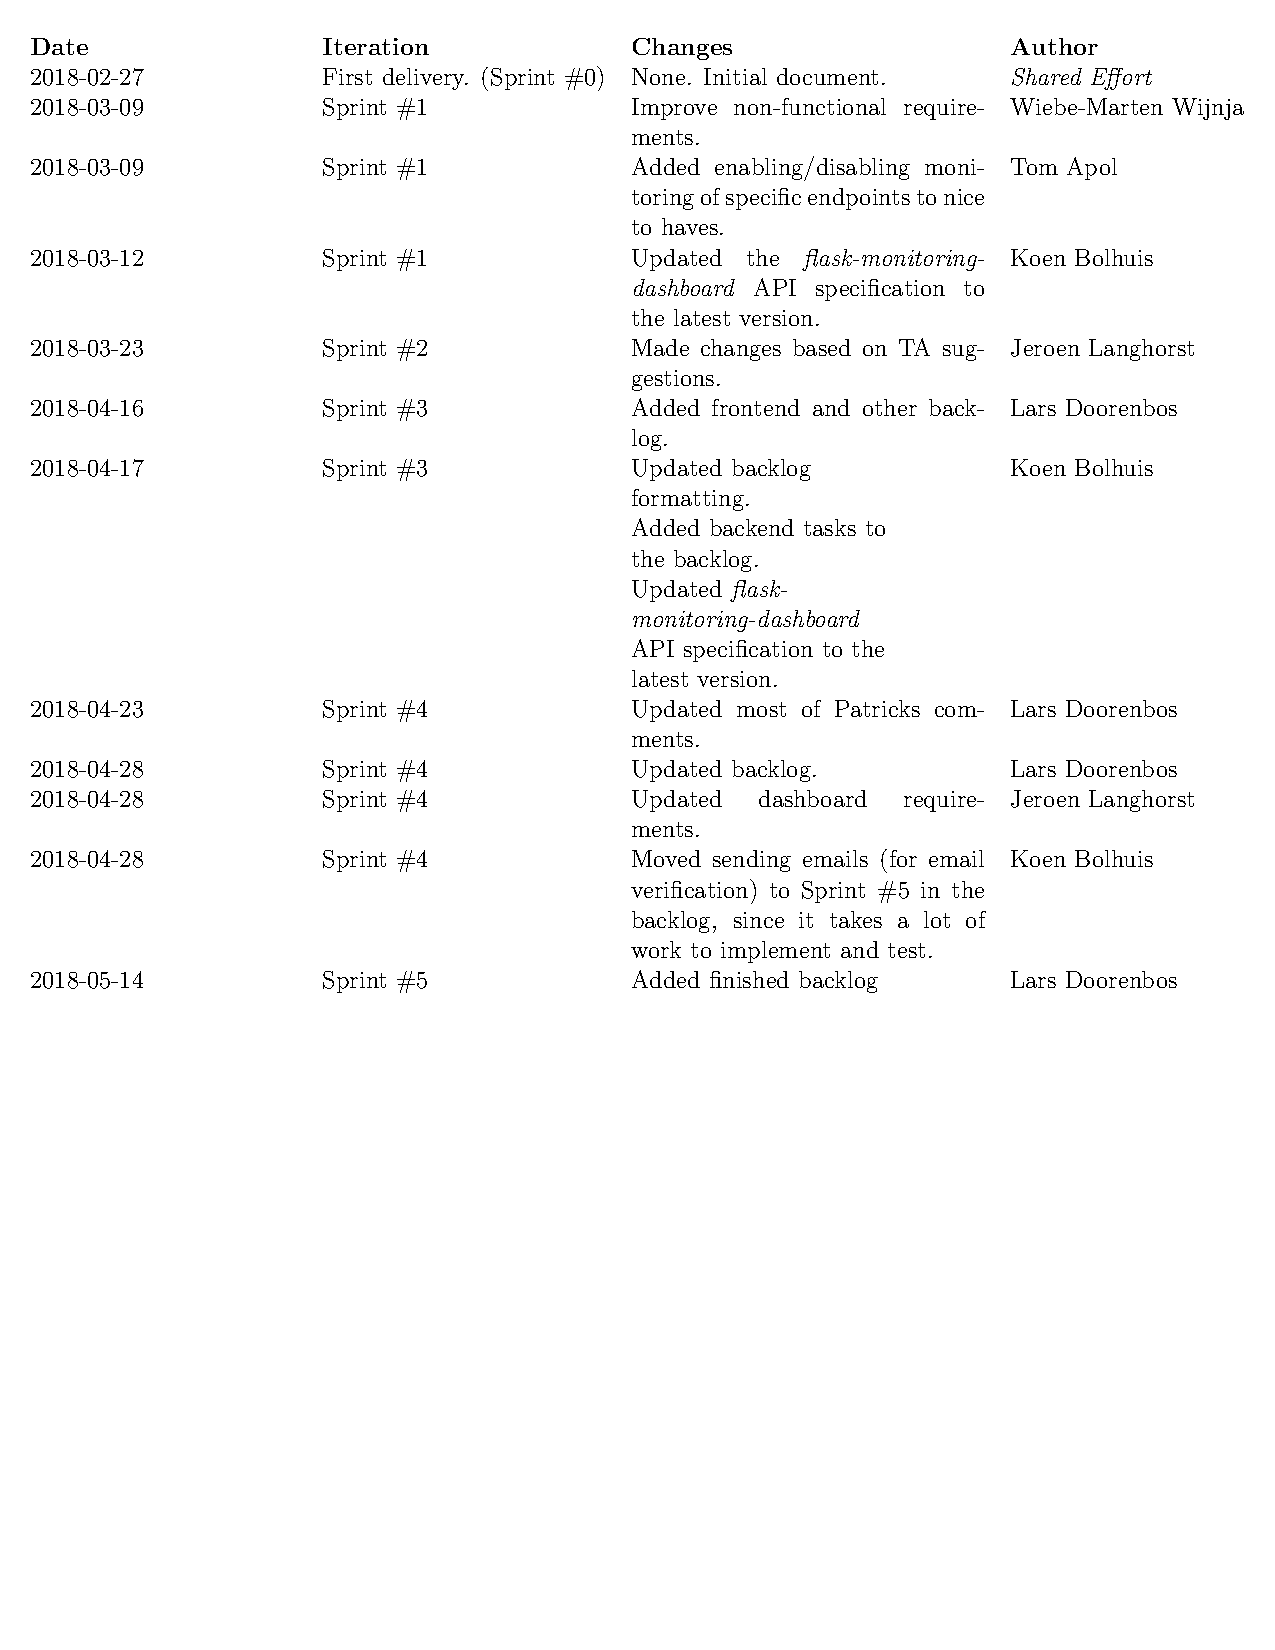
\includegraphics[width=2*\pagewidth]{changelog_requirements.pdf}
